\begin{figure*}[t]
    \centering
    
\includegraphics[width=\textwidth]{images/collage.png}
    \caption{Qualitative overview of EPIC-KITCHENS-100 with multiple example frames illustrating different kitchens, viewpoints and activities. Not all frames have an active action segment (shown as the action labeled below each frame).}
    \label{fig:dataset_collage}
\end{figure*}

\section{Data exploration and description}

In this work we use the EPIC-KITCHENS-100 dataset, focusing on the Multi-Instance Retrieval (MIR) challenge, which provides trimmed egocentric action segments paired with English narrations recorded in 45 kitchens and totalling 100 hours of Full HD video (around 20M frames in 700 variable-length sequences). Videos were captured with head-mounted cameras in the participants' own kitchens, yielding non-scripted multi-day recordings with 97 verb classes and 300 noun classes, making EPIC-KITCHENS-100 the largest egocentric kitchen dataset currently available.

\subsection{Qualitative overview}

Figure~\ref{fig:dataset_collage} shows a collage of frames collected from the official EPIC-KITCHENS resources, illustrating the diversity of kitchens, participants and activities. The examples highlight the strongly egocentric viewpoint, the presence of hands and manipulated objects, and the substantial variation in illumination and background clutter.

\subsection{Video-level characteristics}

The analysis relies on the official file \texttt{EPIC\_100\_video\_info.csv}, which stores per-video duration, frame rate (\texttt{fps}) and spatial resolution (\texttt{width}~$\times$~\texttt{height}). Across the 700 recordings, the mean video duration is approximately 514\,s (8.6\,min) with a standard deviation of 599\,s, ranging from short clips of about 10\,s to long sessions of more than 1\,h (maximum 3708\,s). The average frame rate is 55.9\,fps, with most videos recorded either at 50\,fps or 59.94\,fps, and a few legacy sequences at 29.97, 48 or 90\,fps.

Videos are predominantly recorded at a resolution of \(1920\times1080\) pixels: this Full HD configuration accounts for 694 of the 700 videos, while only four clips use \(1280\times720\) and two use \(1920\times1440\). From this dominant resolution we obtain an average of approximately \(2.07\times10^{6}\) pixels per RGB frame; the distribution of pixels per frame has mean \(2.07\times10^{6}\) and interquartile range concentrated exactly at \(1920\times1080\), with a minimum of \(9.22\times10^{5}\) and a maximum of \(2.76\times10^{6}\) pixels. The empirical distributions of video duration and frame rate are visualised in Figure~\ref{fig:video_duration_fps}, showing that most sequences cluster around medium-length recordings at 50--60\,fps, with a long tail of very long videos.

\begin{figure}[h]
    \centering
    \begin{subfigure}[b]{0.48\columnwidth}
        \centering
        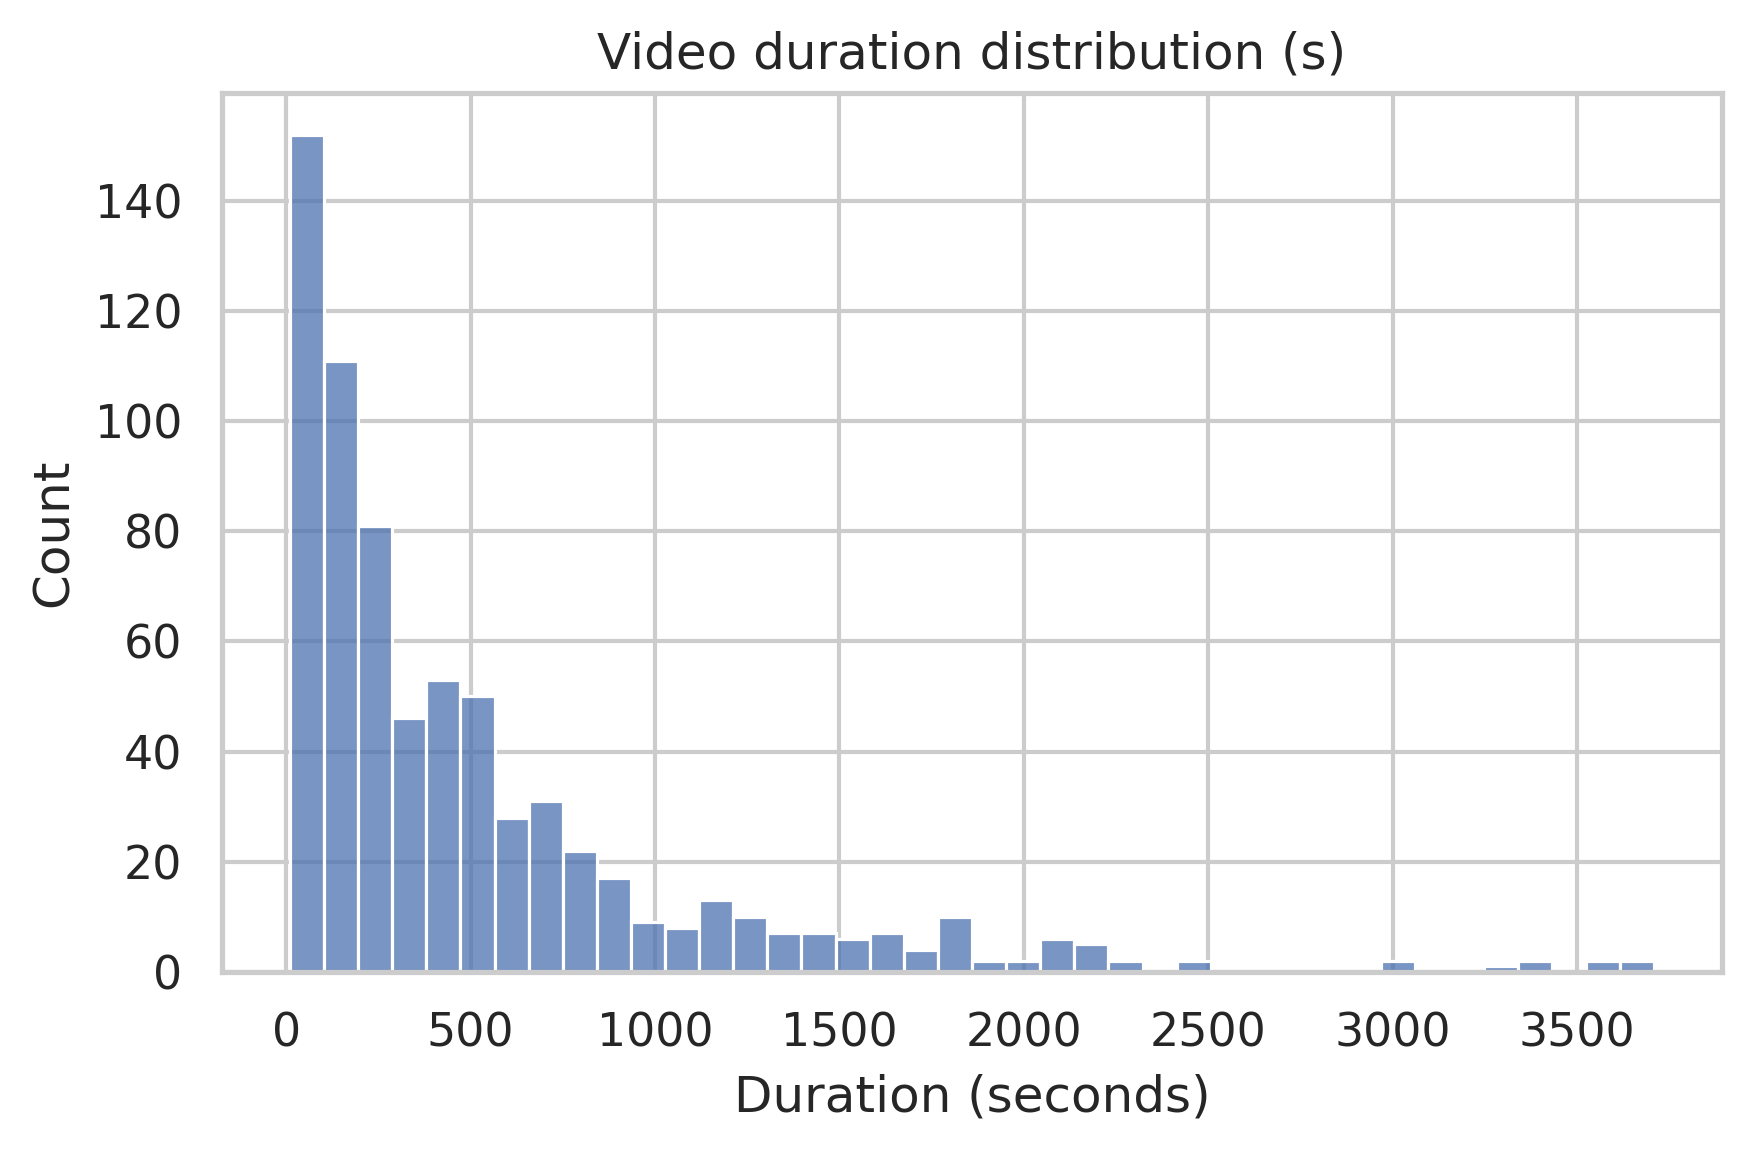
\includegraphics[width=\columnwidth]{images/video_duration_hist.png}
        \caption{Video duration.}
        \label{fig:video_duration_hist}
    \end{subfigure}
    \hfill
    \begin{subfigure}[b]{0.48\columnwidth}
        \centering
        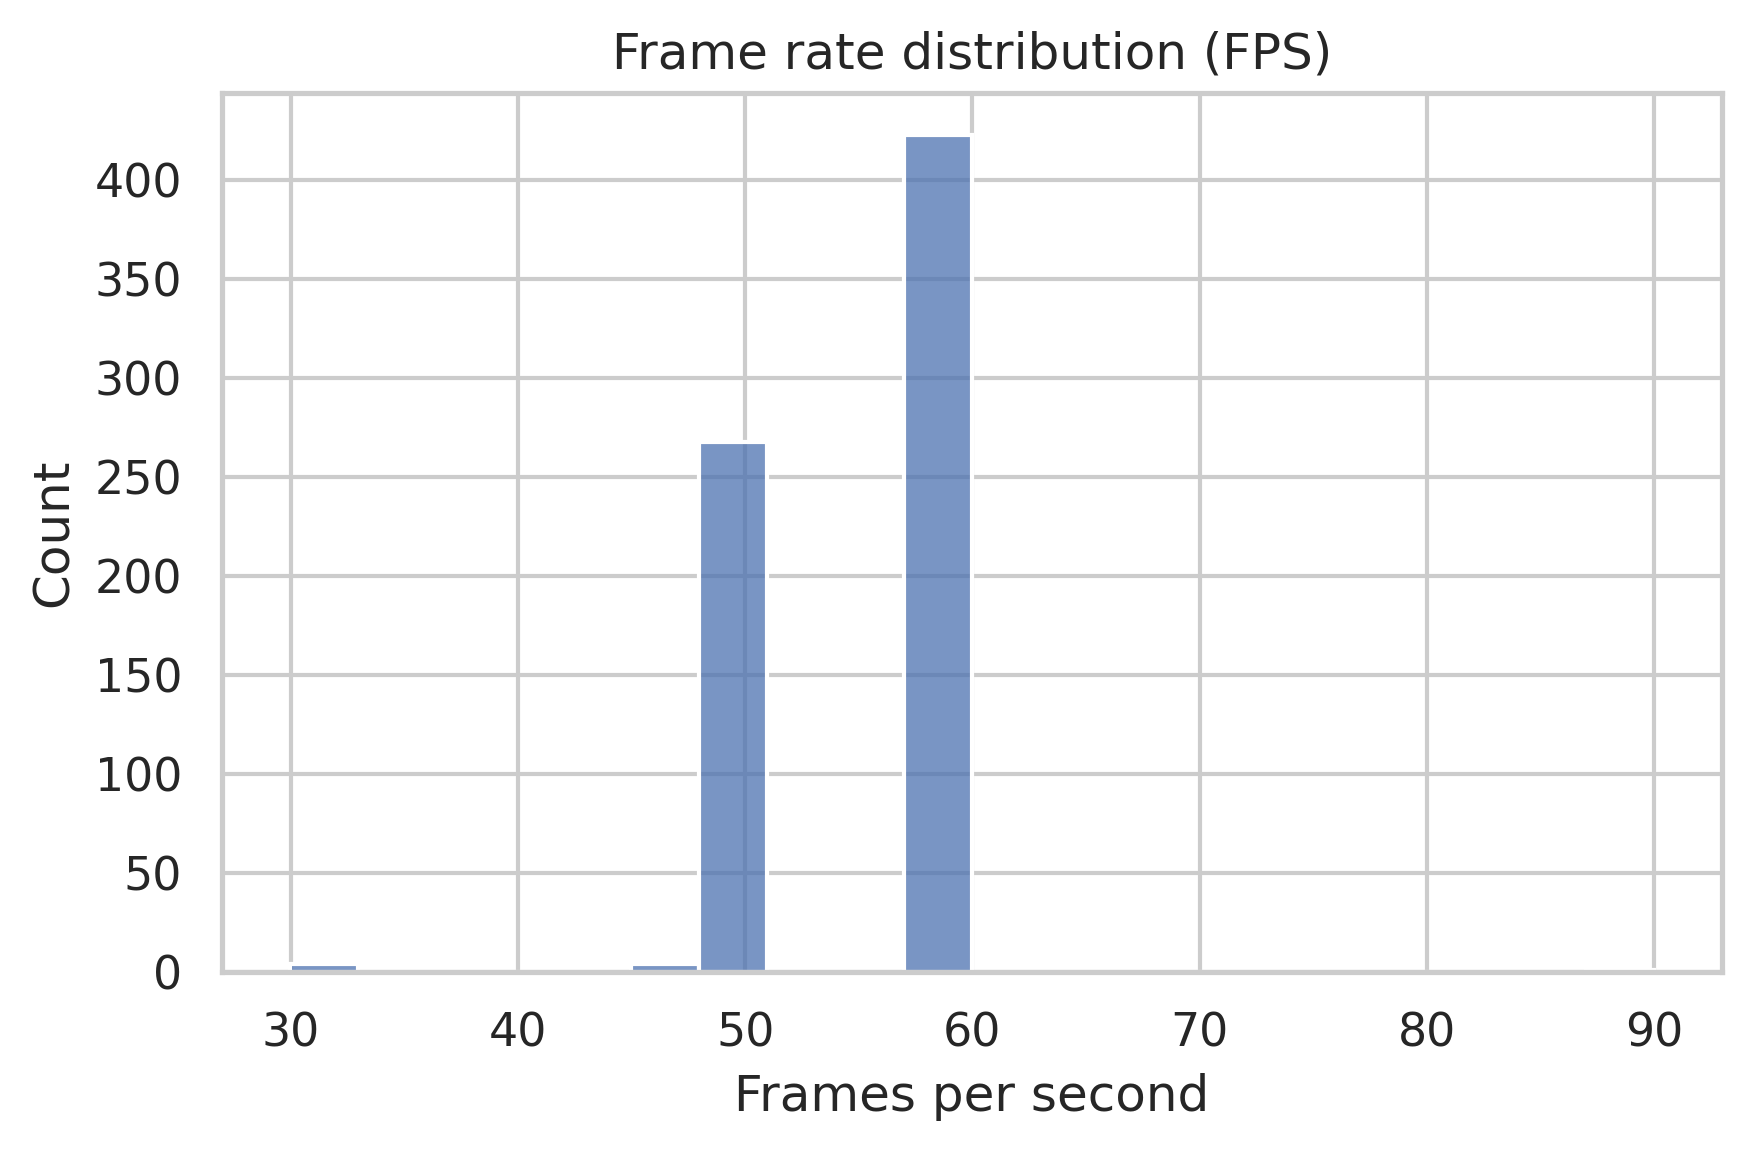
\includegraphics[width=\columnwidth]{images/fps_hist.png}
        \caption{Frame rate.}
        \label{fig:fps_hist}
    \end{subfigure}
    \caption{Video-level distributions of duration (seconds) and frame rate (frames per second) in EPIC-KITCHENS-100. Each plot fits within a single column.}
    \label{fig:video_duration_fps}
\end{figure}

\subsection{Image-level characteristics}

For each action segment in the MIR train and test splits, frame-level properties are derived by combining the segment start and stop frames with the per-video resolution and \texttt{fps} metadata. Because the underlying videos are almost entirely Full HD, the distribution of frame sizes is sharply peaked at \(1920\times1080\) pixels, and the average number of pixels per frame across the MIR subset closely matches the dataset-wide value of approximately 2.07\,M pixels. Although we omit the corresponding plot for space reasons, the histogram of total pixel counts confirms that 75\% of the frames lie exactly at the Full HD resolution, with only a handful of frames at the two alternative resolutions mentioned above.

To characterise appearance statistics, a subset of 1000 RGB frames is sampled uniformly from the MIR training split, using frames pre-extracted with the official download scripts. For each sampled frame we compute the mean and standard deviation of pixel intensities in RGB space; on average, the overall mean intensity is 0.39 (on a 0--1 scale) with standard deviation 0.06, while the per-channel means are approximately 0.44 (R), 0.37 (G) and 0.36 (B) with per-channel standard deviations around 0.21. The resulting distributions, shown in Figures~\ref{fig:mean_intensity_hist} and~\ref{fig:channel_stats_boxplot}, summarise typical illumination levels and highlight the variability induced by different kitchens and recording days. A representative EPIC-KITCHENS frame from this subset is also shown in Figure~\ref{fig:example_frame}, illustrating the egocentric viewpoint, field of view and typical cluttered kitchen environment.

\begin{figure}[h]
    \centering
    \begin{subfigure}[b]{0.48\columnwidth}
        \centering
        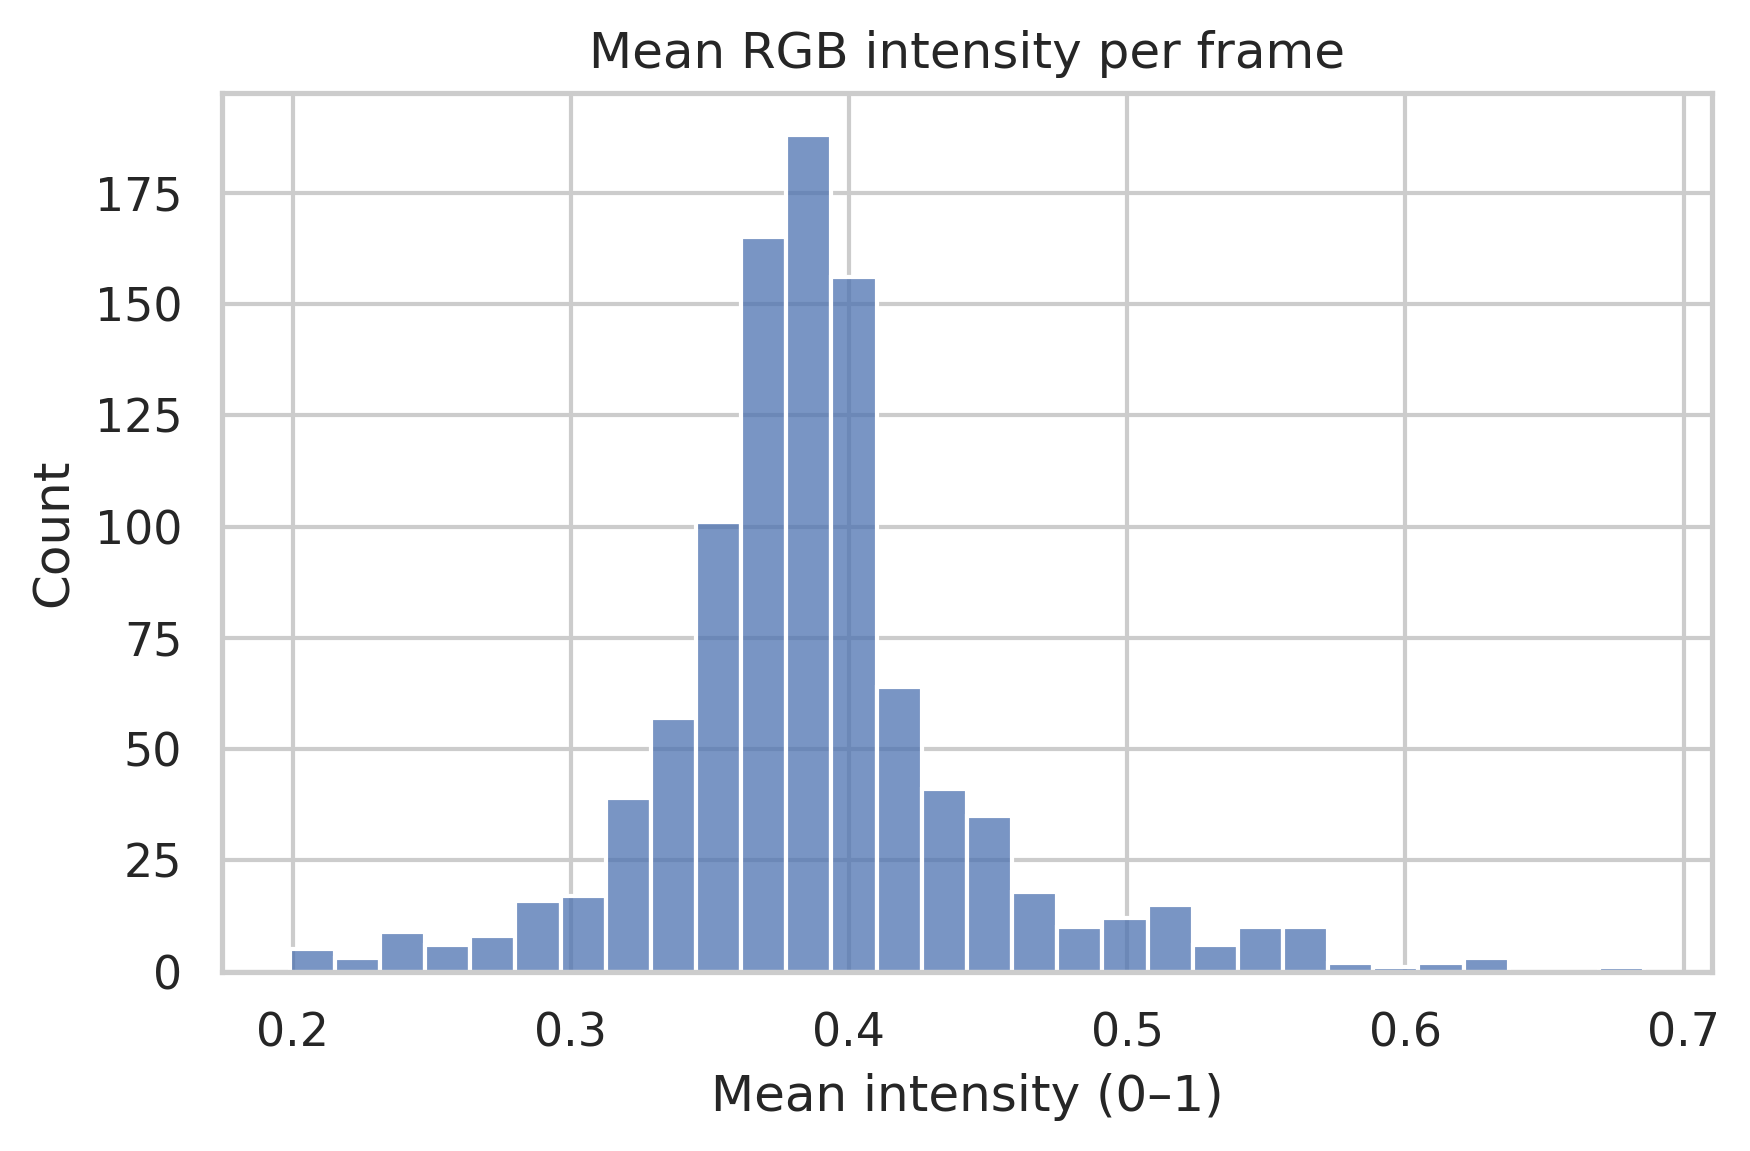
\includegraphics[width=\columnwidth]{images/mean_intensity_hist.png}
        \caption{Mean intensity.}
        \label{fig:mean_intensity_hist}
    \end{subfigure}
    \hfill
    \begin{subfigure}[b]{0.48\columnwidth}
        \centering
        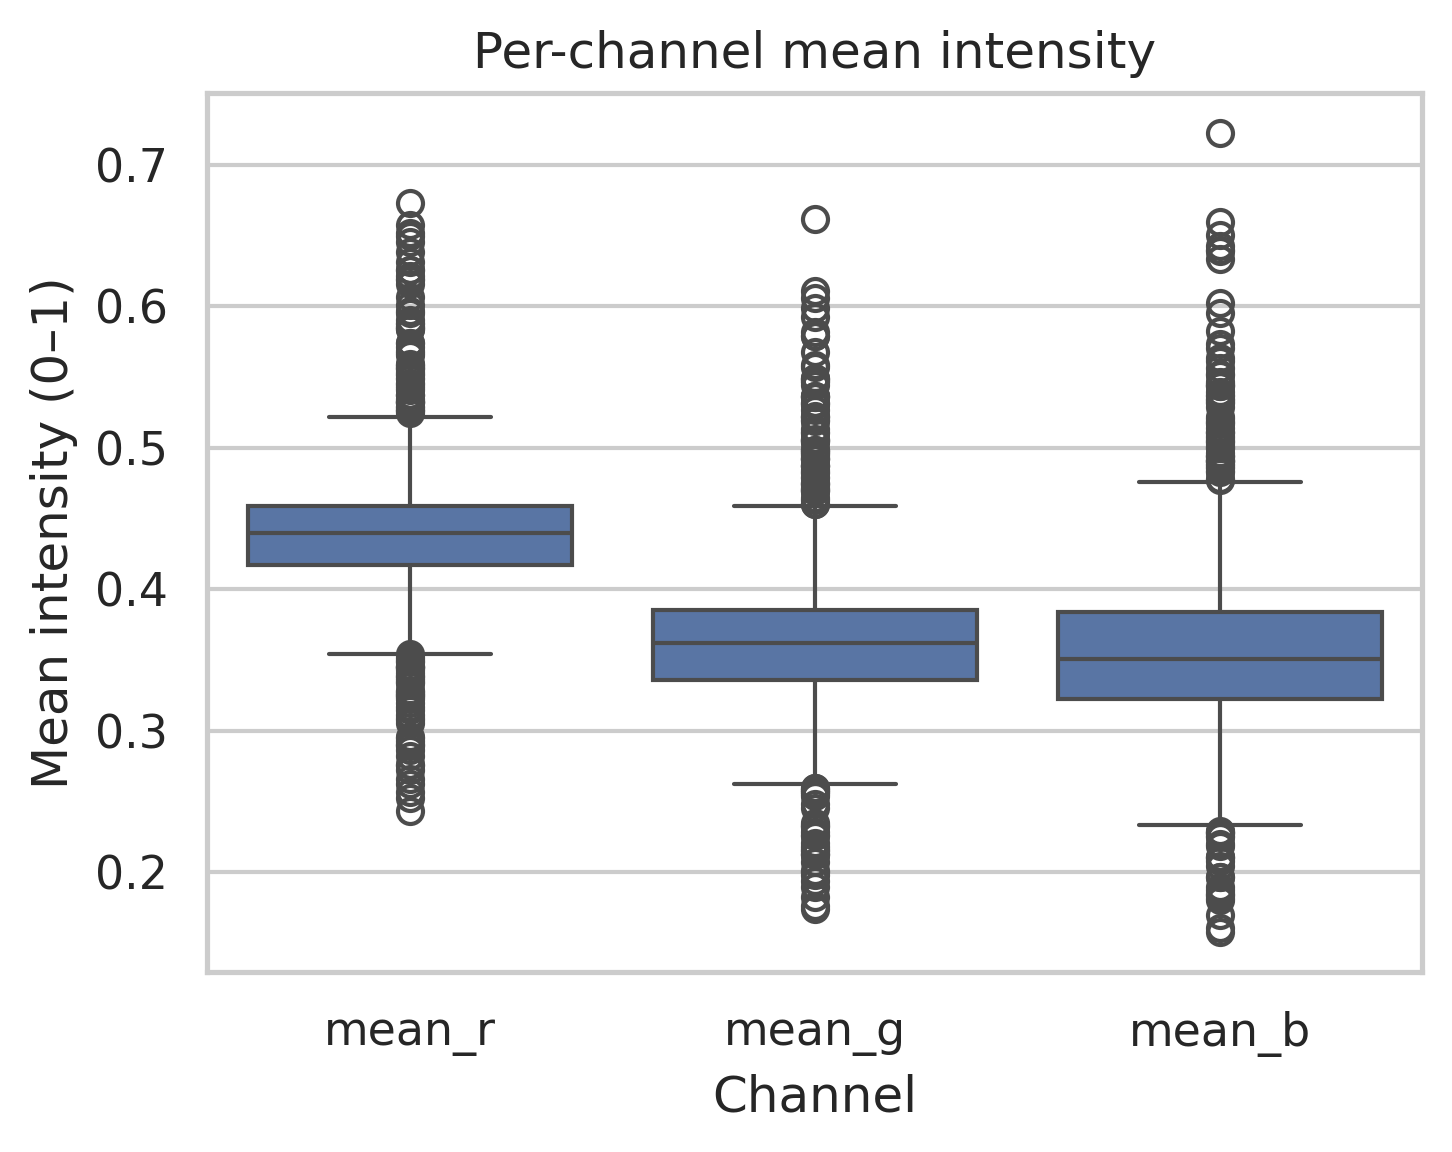
\includegraphics[width=\columnwidth]{images/channel_stats_boxplot.png}
        \caption{Per-channel means.}
        \label{fig:channel_stats_boxplot}
    \end{subfigure}
    \caption{Image-level appearance statistics computed from a subset of RGB frames. Left: histogram of mean RGB intensity per frame. Right: box plots of per-channel mean intensity.}
    \label{fig:intensity_stats}
\end{figure}

\subsection{Segment-level statistics for MIR}

The MIR challenge operates on trimmed action segments with associated narrations rather than full untrimmed sequences, so we also explore statistics at the segment level using the retrieval annotation files \texttt{EPIC\_100\_retrieval\_train.csv} and \texttt{EPIC\_100\_retrieval\_test.csv}. Each row provides a unique segment identifier, the \texttt{video\_id}, and the corresponding \texttt{start\_frame} and \texttt{stop\_frame}. By combining these with the per-video \texttt{fps} values, we compute the duration of each segment in seconds as \(\texttt{duration} = (\texttt{stop\_frame} - \texttt{start\_frame} + 1)/\texttt{fps}\). 

For the 67{,}217 MIR training segments, the mean duration is 3.18\,s with a standard deviation of 5.53\,s, a median of 1.6\,s and an interquartile range between 1.0 and 3.18\,s, confirming that most MIR clips are very short. At the same time, the maximum segment lasts almost 5\,min (297\,s), evidencing a long tail of extended actions that provide additional temporal context. 

\begin{figure}[h]
    \centering
    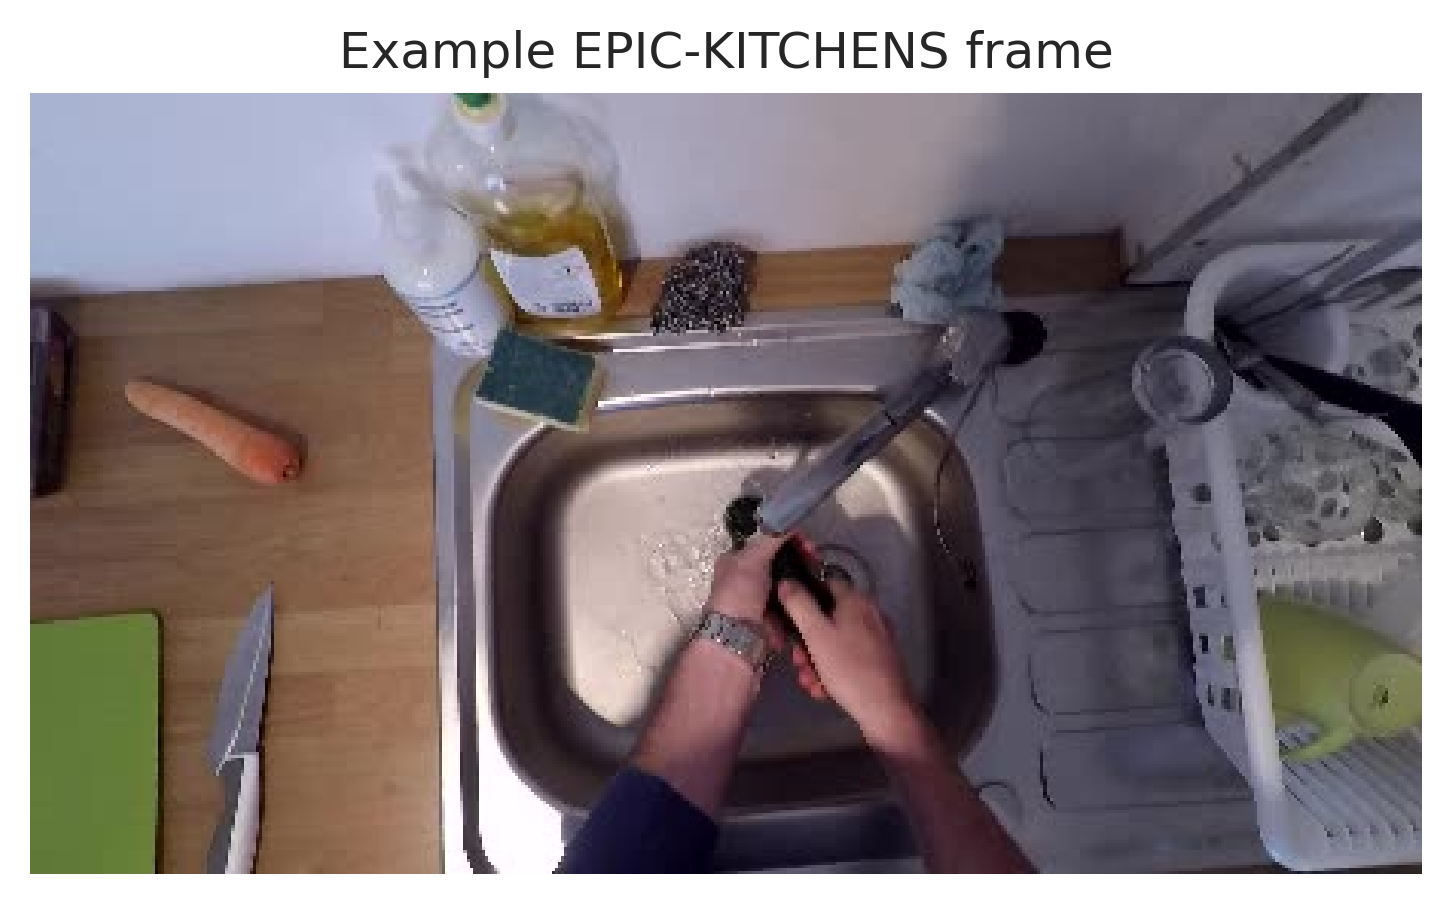
\includegraphics[width=\columnwidth]{images/example_frame.png}
    \caption{Example EPIC-KITCHENS frame from the MIR training split, showing the egocentric viewpoint and typical visual clutter.}
    \label{fig:example_frame}
\end{figure}
